%=====================================================================================================================
\section{Rollouts relax toward a conditioning-set default}\label{sec:relax}

\paragraph{Tone.} Observationally, the 31-s change of every global statistic is anti-correlated with its opening value
($r$ from $-0.79$ to $-0.95$; Appendix Table~\ref{tab:attr}), but openings differ in content too, so we intervened: we
shifted the brightness and colour temperature of the same opening within each of 24 scenes (12 NAVSIM, 12 generated)
and continued every version with the generic prompt (study 6, 31\,s; study 10, 60\,s). The versions converge
(Fig.~\ref{fig:teaser}). At 60\,s every cache configuration has relaxed (Fig.~\ref{fig:atlas}a): $\alpha$ ranges from
$-0.01$ (LongLive without a sink) to 0.79 (Self Forcing GAN), ranked as at 31\,s (Spearman $\rho=0.78$, $p=0.008$).
Part of the loss is immediate: most configurations lose a fifth to a third of the shift within 4.5\,s, and SiD loses
almost all of its total there (0.66 of 0.65), which looks like the model rejecting an off-manifold shift rather than
forgetting it. Colour temperature behaves like brightness. Persistence varies by checkpoint even with architecture,
context and sampler fixed (Self Forcing: 0.35 to 0.79 at 60\,s; two SiD checkpoints differ by 0.36), so it is a
property of the checkpoint rather than of the training objective.

\paragraph{The response is linear in the shift.} Equation~\ref{eq:law} treats $\alpha$ as independent of how far the
opening was shifted, but every $\alpha$ above comes from one pair of shifts ($\pm16$~\Lstar). Study 23 shifted the same
24 openings by $-24$, $-8$, 0, $+8$ and $+24$~\Lstar{} (Self Forcing, 60\,s, two seeds, 720 videos) and tested
equivalence within $\pm0.15$. \pend{[results: large vs small shift with sink, re-rotated sink; darkening vs
brightening; no sink forgets a large shift too.]} In study 6, persistence from $\pm8$ and from $\pm16$ shifts agrees
within 0.09 in 12 of 14 configurations at 31\,s (exploratory; Appendix~\ref{app:robust}).

\begin{figure}[t]
\centering
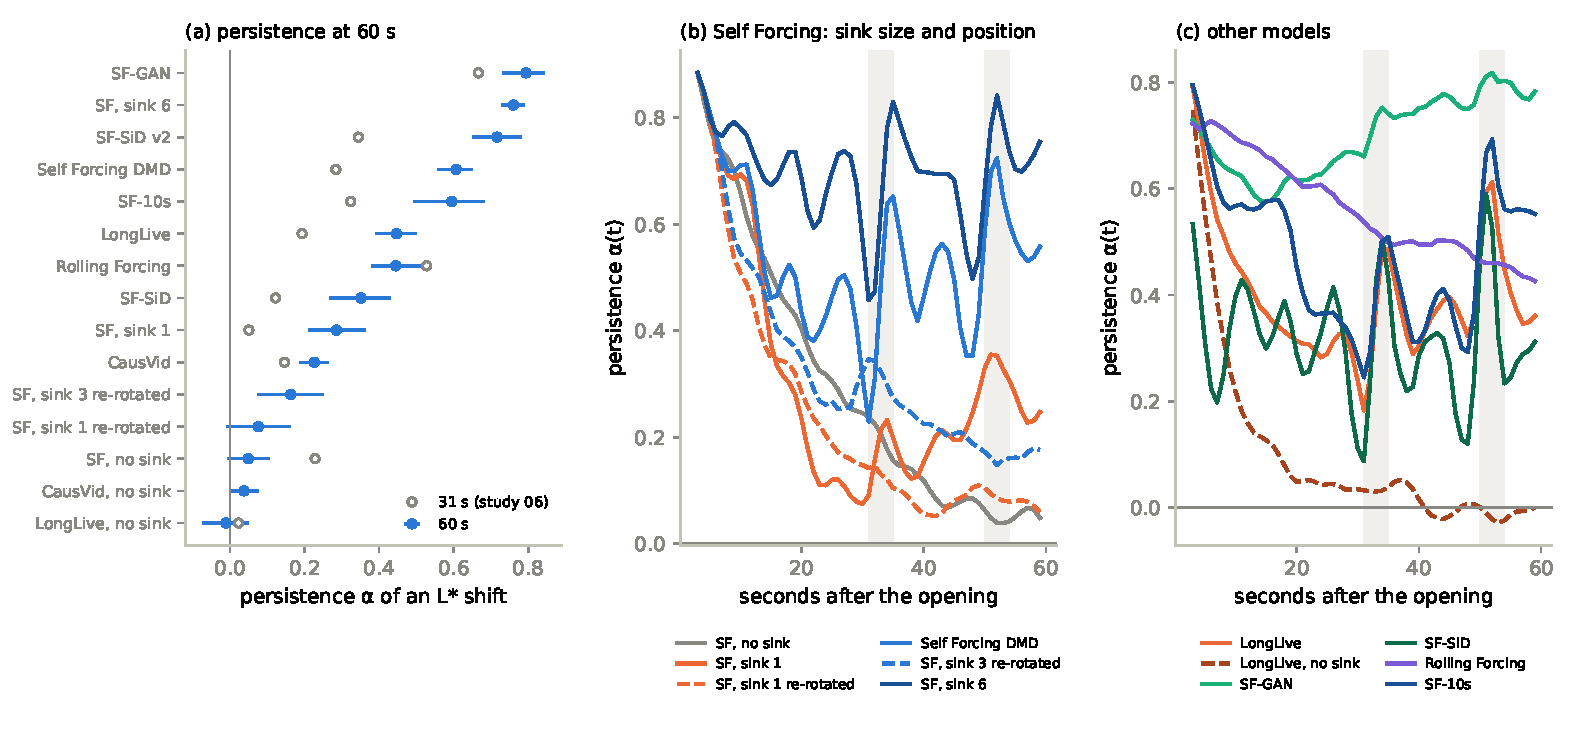
\includegraphics[width=\linewidth]{fig_atlas.pdf}
\caption{Persistence at 60\,s (study 10; CausVid from study 7). (a) $\alpha$ of an \Lstar{} shift with
scene-bootstrap 95\% CIs; hollow markers: 31\,s (study 6). (b) Self Forcing with sinks of 0, 1, 3 and 6 latent frames,
at their original positions or re-rotated to sit just before the window (dashed). (c) Other models. Curves: 1-s windows,
3-s moving average; shaded: 31--35\,s and 50--54\,s, where sinks of three or more frames at their original positions
produce bursts. The 60-s endpoint window, [50, 60)\,s, overlaps the second burst; Appendix~\ref{app:robust} reports a
burst-free window.}
\label{fig:atlas}
\end{figure}

\subsection{Scene content}\label{sec:content}
Global tone is the easiest statistic to shift and measure, but it is not what a user sees as ``the scene''. We
therefore generated openings of six scene classes (snow, desert, forest, coast, mountain, farmland; four each, selected
by CLIP before any continuation) and continued each under the generic city prompt and under its own class prompt, with
eight configurations (study 9). Content relaxes like tone (Fig.~\ref{fig:content}). Under the city prompt, $\kappa$ at
30\,s ranges from 0.07 (SiD) to 0.61 (Rolling Forcing), and the opening's class is CLIP's top label in only 34\% of Self
Forcing frames at 30\,s. Under the opening's own class prompt the class persists ($\kappa$ 0.71--1.05; 9.3
\ci{8.1}{10.5} more log-odds than under the city prompt, preregistered), as a fresh rollout of that prompt would also
show it; the informative result is the loss under the city prompt. Content and tone persistence are correlated across
configurations ($\rho=0.67$, $p=0.07$, $n=8$).

Sinks act differently on content. Self Forcing's sink keeps more of it at 60\,s ($\kappa$ 0.61 vs 0.14, $+0.48$
\ci{0.39}{0.57}, preregistered), but not steadily: $\kappa$ falls to 0.32 at 30\,s and rises again, and the dunes, the
sea and the mountains of the opening reappear after a minute of city (Fig.~\ref{fig:content}, left). The returns are
positional (study 16, 24 openings): with the sink's keys re-rotated to sit just before the window, they vanish (burst
contrast $-0.29$ \ci{-0.37}{-0.22}), and the content kept at 60\,s falls from 0.56 to 0.25 ($-0.31$
\ci{-0.37}{-0.25}). With this one seed the re-rotated sink kept no detectably more content than no sink ($+0.10$
\ci{-0.00}{0.21}, not supported). Three new seeds per opening (study 21, 240 videos) reproduce the sink's advantage,
the loss under re-rotation ($-0.40$ \ci{-0.47}{-0.34}) and the positional return, and, averaged per opening, detect a
small share kept by the re-rotated sink: 0.19 against 0.11 without a sink ($+0.08$, Holm $p=0.006$; \ci{-0.01}{0.16}
when the fresh starts are also resampled). What a Self Forcing sink keeps of the scene, it keeps mostly by periodically
re-injecting the opening. LongLive's sink, which keeps tone, does not keep content (0.22 vs 0.24, preregistered test not
supported).

Content relaxes outside the Wan-1.3B family too. FramePack, continuing the same 24 openings under the city prompt,
keeps 0.55 of the class evidence at 20\,s (Self Forcing: 0.40 with a sink, 0.31 without; study 17). Giving its two
routes different images separates them (Appendix Fig.~\ref{fig:framepack}b): the clean context prefix alone keeps 0.24
\ci{0.12}{0.37}, levelling off after 14\,s, while the SigLIP image embedding alone, with a city frame in the context,
\emph{pulls} the video toward the opening's class, to 0.23 \ci{0.16}{0.30} at 20\,s and still rising. The same
embedding has no effect on tone (study 11), so in FramePack it sets the default of the scene but not of its
brightness. \pend{[Krea 14B (study 22) and MAGI-1 (study 19) content results.]}

\begin{figure}[t]
\centering
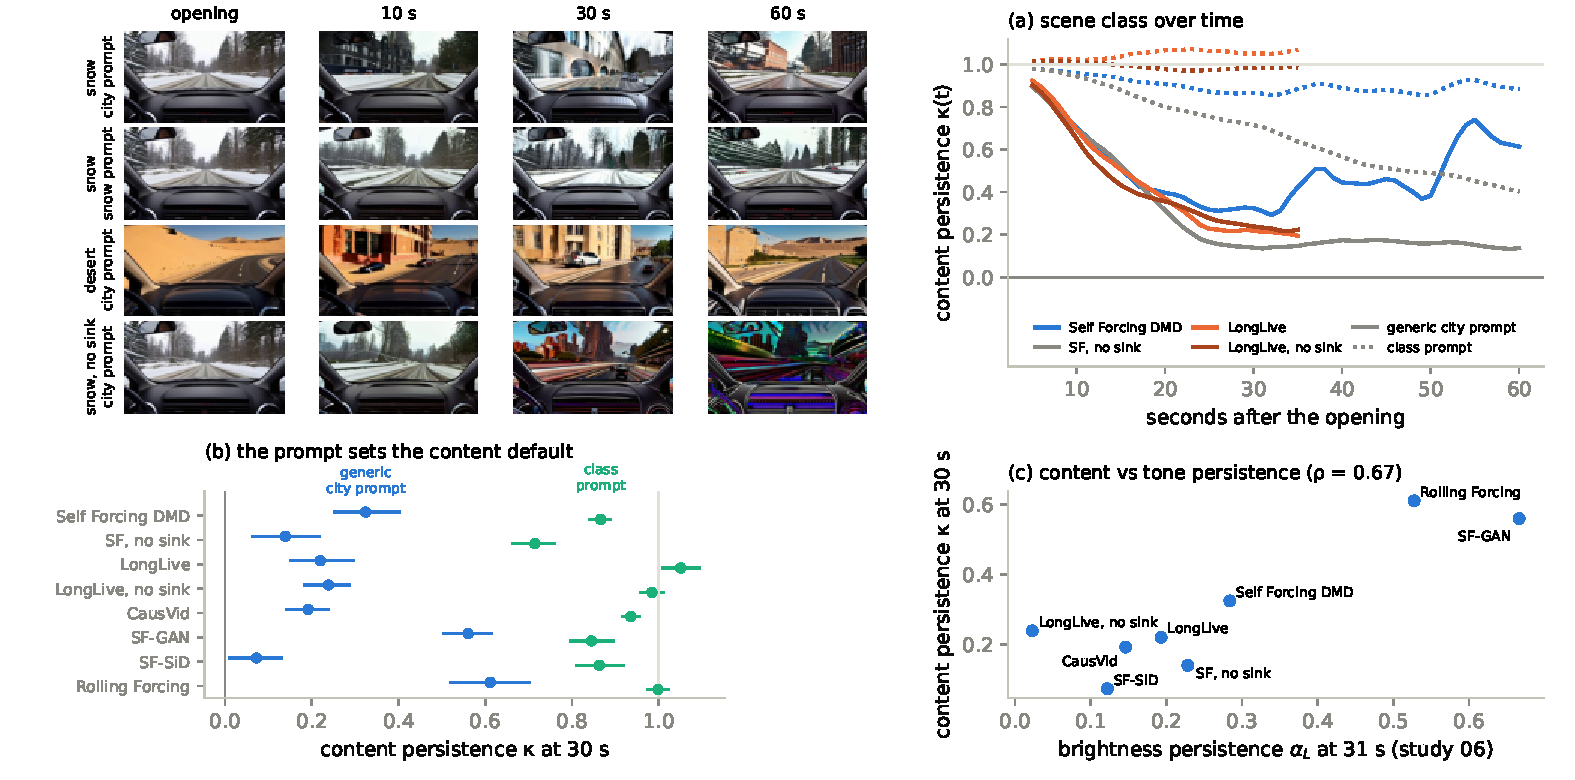
\includegraphics[width=\linewidth]{fig_content.pdf}
\caption{Scene content relaxes to the prompt's default (study 9). Left: a snow and a desert opening continued by Self
Forcing DMD under the city prompt or their own class prompt. Under the city prompt both become city streets; with a
sink the desert returns at 60\,s; without a sink the video collapses. (a) Content persistence $\kappa(t)$ (CLIP
log-odds of the opening's class against ``city street'', 0 = fresh generic rollout, 1 = opening) under the city prompt
(solid) and the class prompt (dotted). (b) $\kappa$ at 30\,s, 24 openings, 95\% CIs. (c) Content against brightness
persistence across configurations.}
\label{fig:content}
\end{figure}

\subsection{The default}\label{sec:default}
\paragraph{The conditioning sets it.} Continuing the same 40 openings under four lighting prompts gives four defaults:
on Self Forcing, sunny 43, overcast 34, dusk 19 and night 16~\Lstar; on LongLive the same words give 45, 40, 32 and 21
(Appendix Fig.~\ref{fig:default}). The mapping from words to brightness is model-specific. Under one prompt the default
also differs between checkpoints of one architecture (zero-drift levels from 17 to 54~\Lstar), and it tracks where
prompt-only rollouts end ($r=0.93$, slope 1.58; Appendix~\ref{app:robust}).

\paragraph{Persistence depends on the scene.} Equation~\ref{eq:law} separates a model term ($\alpha$) from a prompt
term ($\mu$), but $\alpha$ itself varies: Self Forcing keeps 0.34 of the opening under a sunny prompt and 0.05 under a
night prompt (exploratory interaction, $p=0.001$). In four new scene types with their own prompts and self-generated
openings (a park walk, a drone flight over a coast, a kitchen, a market; study 12), its persistence at 60\,s differs
between them (0.44 to 0.67, $p=0.049$, preregistered), as does LongLive's at 30\,s (0.10 to 0.43). The sink effect
replicates almost exactly outside driving scenes: 0.55 with a sink and 0.02 without ($+0.53$ \ci{0.45}{0.61}).

\paragraph{Two components of drift.} For a prompt-only rollout, Eq.~\ref{eq:law} says nothing about why the default
should differ from where the same prompt starts. It does, and by how much depends on training (Appendix
Fig.~\ref{fig:mech}a). Fresh rollouts of Self Forcing (trained on its own 5-s rollouts) and CausVid end 4--11~\Lstar{}
from where they start; those of LongLive and Rolling Forcing, trained or tuned on their own long rollouts, 0.7--2.3~\Lstar.
Yet LongLive still forgets its opening ($\alpha=0.02$ without a sink at 31\,s). In this exploratory analysis drift has
two separable parts: \emph{forgetting} the opening, $(1-\alpha)(x_{\text{open}}-\mu)$, which every attention-based
model does, and an \emph{attractor offset} $\mu - x_{\text{start}}$, which is near zero in the two models trained on
their own long rollouts (other differences between them and the short-clip models cannot be excluded). \pend{[fresh
offsets of Krea and MAGI-1.]} Prompt-only drift metrics mix the two, and both keep rising over 31\,s even with a sink
(Appendix~\ref{app:ctx}); relaxation describes the memory of the opening, not the absence of degradation.

%=====================================================================================================================
\section{What decides how much of the opening is kept}\label{sec:mech}
Figure~\ref{fig:hold} collects the long-run persistence of every model and configuration we ran for 60\,s, grouped by
how the model holds the opening. Four regimes appear. An opening seen only through a sliding key--value window is
forgotten. Re-denoising overlapping frames passes it forward and delays forgetting by about 20\,s. An opening kept
next to the window, at positions of the kind the model was trained on, holds a steady share whose size depends on the
model. A sink at its original rotary positions keeps the most, but largely through periodic positional bursts.

\begin{figure}[t]
\centering
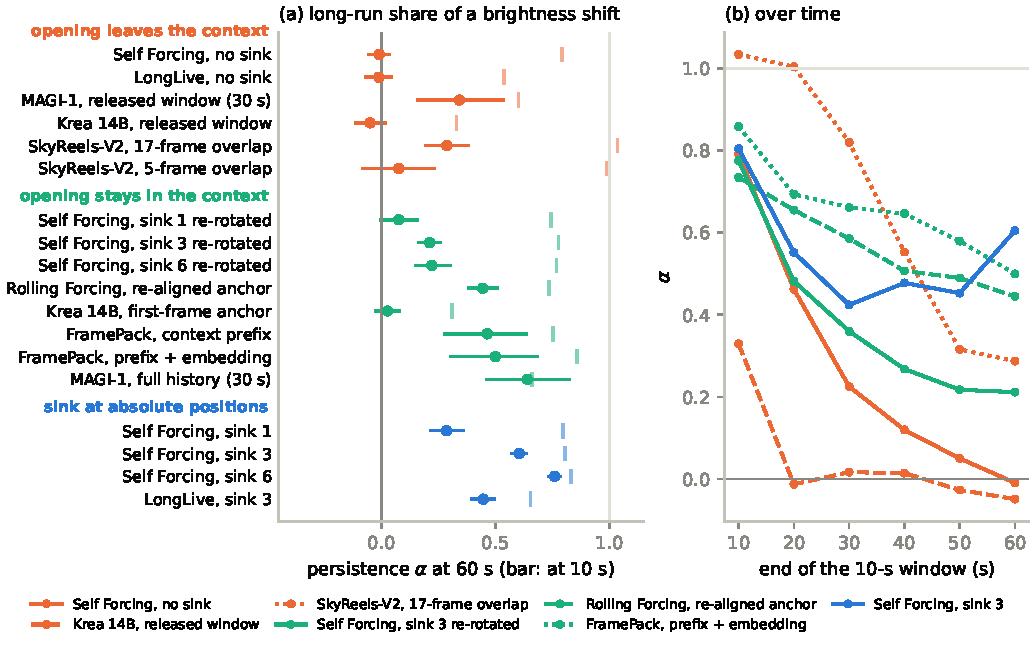
\includegraphics[width=\linewidth]{fig_hold.pdf}
\caption{How the opening is held decides how much of it is kept. (a) Persistence of an \Lstar{} shift at 60\,s
(window [50, 60)\,s; MAGI-1 full history: 30\,s) with scene-bootstrap 95\% CIs; ticks: at 10\,s. (b) Persistence
over time (10-s windows) for one configuration per regime.}
\label{fig:hold}
\end{figure}

\paragraph{Only in the window: forgotten.} Without a sink, Self Forcing and LongLive keep 0.05 and $-0.01$ at 60\,s
(study 10). MAGI-1~\cite{magi} (4.5B, distilled), which shares neither architecture nor training with the other models,
attends in its released configuration to the four previous 1-s chunks, so the opening leaves its context after about
4\,s; persistence falls from 0.87 at 5\,s to 0.34 at 30\,s ($-0.52$ \ci{-0.70}{-0.35}, study 18)
\pend{and to [x] at 60\,s (study 19)}. Krea Realtime 14B~\cite{krea}, Self Forcing distilled from Wan2.1-14B and ten
times the size of the other Wan models, recomputes its cache over a window of three latent frames (study 22, 24 scenes):
\pend{it keeps 0.33 at 10\,s and nothing from 20\,s on ($-0.05$ at 60\,s)}. Scale does not change the regime.

\paragraph{Sinks: depth helps only at the original positions.} In study 6, removing LongLive's sink lowered $\alpha$
at 31\,s from 0.19 to 0.02 ($-0.17$ \ci{-0.28}{-0.06}); for Self Forcing the preregistered test failed at 31\,s
($-0.06$ \ci{-0.17}{0.05}) because without a sink it forgets slowly (Fig.~\ref{fig:atlas}b). At 60\,s the difference is
large (studies 7, 10): no sink 0.05, a sink of one latent frame 0.29, three 0.61, six 0.76 ($+0.15$ \ci{0.11}{0.20}
for six vs three), and 0.45 against $-0.01$ for LongLive. The sink's \emph{position} matters more than its depth. Self
Forcing keeps the sink keys at their absolute rotary positions, ever further from the current chunk; re-rotating them
to sit just before the window, as Rolling Forcing and Deep Forcing do, lowers persistence at 60\,s from 0.61 to 0.16
($-0.44$ \ci{-0.54}{-0.35}, preregistered; 40--50\,s, between the bursts: $-0.27$ \ci{-0.38}{-0.16}). Re-rotated, depth
no longer helps (study 16): sinks of six and three frames keep the same share (0.22 vs 0.23, $-0.00$ \ci{-0.11}{0.10};
the preregistered depth test is not supported), and their curves coincide from 10\,s on. Three new seeds per scene
(study 20, 432 videos) reproduce this: 0.61 with a sink, 0.21 re-rotated and $-0.01$ without, the re-rotated sink
keeping more than none ($+0.22$ \ci{0.15}{0.29}), in each seed alone too. Krea's optional first-frame anchor, one
latent frame kept next to the window, keeps \pend{0.03 at 60\,s ([test A3])}, like a re-rotated one-frame sink on Self
Forcing (0.08). A sink at in-distribution positions thus holds a small, steady share of tone, at most about 0.2 whatever
its depth, and a smaller share of the scene (Section~\ref{sec:content}).

\paragraph{Sinks at their original positions: bursts.} Persistence with such a sink jumps between 31.5 and 34.5\,s
($+0.45$ \ci{0.36}{0.53} with three frames, $+0.46$ with six) and again near 52\,s, in LongLive and the other Self
Forcing checkpoints too (Fig.~\ref{fig:atlas}b, c); the returns of the opening's scene coincide with these bursts. With
re-rotated sinks the jump is replaced by a small decline ($-0.08$ \ci{-0.13}{-0.02}). The timing matches the ``sink
collapse'' that LoL~\cite{lol} attributes to rotary-position periodicity, and the role of intrinsic rotary frequencies
in video length extrapolation~\cite{riflex,roundround}: the sink keeps its absolute position, and at certain distances
the current chunk attends to it strongly. Much of what a Self Forcing sink keeps at 60\,s is therefore positional.

\paragraph{Overlapping frames delay forgetting.} SkyReels-V2-DF extends videos in 97-frame segments that re-denoise
the last 17 frames of the previous segment jointly with the new ones. It does not relax over 20\,s ($\alpha = 0.96$
\ci{0.86}{1.07}), whatever its guidance, history noise or number of steps (exploratory), and in 5 of 12 scenes
$\alpha>1$: the overlap passes the opening forward and can amplify it. Cutting the overlap to 5 frames makes it relax
($-0.24$ \ci{-0.40}{-0.09} at 15--20\,s, preregistered). But the overlap only passes the opening forward: over 60\,s
(study 16) 17 frames hold $\alpha\approx1$ until 20\,s and then forget steadily, to 0.29 at 60\,s ($-0.72$
\ci{-0.81}{-0.63} from 20 to 60\,s), and 5 frames fall to 0.08 (both preregistered).

\paragraph{A copy of the opening in every section is a permanent sink.} FramePack~\cite{framepack}, a 13B model
fine-tuned from HunyuanVideo~\cite{hunyuan}, places the opening as a clean prefix frame in the context of \emph{every}
33-frame section and also feeds its SigLIP embedding as a global condition (study 11, 12 scenes). It relaxes too: 0.91
of a brightness shift at 5\,s and 0.68 \ci{0.57}{0.79} at 20\,s (preregistered), about as much as the best cache
configurations over the same window (Appendix Table~\ref{tab:matched}). The shift travels through the prefix: sent
only through the prefix it keeps about half, only through the embedding nothing (0.01 \ci{-0.14}{0.17}). Unlike the
overlap, the prefix keeps its share: at 60\,s (study 16) FramePack keeps 0.51 \ci{0.29}{0.71} with both routes and
0.46 \ci{0.28}{0.65} with the prefix alone, with little decline after 20\,s ($-0.17$ \ci{-0.38}{0.01} and $-0.08$
\ci{-0.26}{0.09}; one collapsed scene excluded). MAGI-1 with full history, the opening never leaving the context,
behaves alike: its persistence levels off near 0.65 from 10\,s on (0.64 \ci{0.45}{0.83} at 30\,s, $+0.30$
\ci{0.17}{0.43} over the released window). Keeping the opening does not stop the shared drift, though: MAGI-1's fresh
rollouts brighten by 15--20~\Lstar{} under either setting, so full history preserves the difference between openings,
not their level.

\paragraph{An action-conditioned world model.} Matrix-Game-2.0~\cite{matrixgame2} generates a world from an image and
keyboard and mouse actions, with no text; the opening's latent leaves its 6-frame window after about a second, while
its CLIP~\cite{clip} embedding conditions every chunk (study 15). The model often collapses to black (40 of 144 videos
within 30\,s), which left 7 scenes for the preregistered 30-s analysis: a shift held only in the context faded ($-0.24$
\ci{-0.35}{-0.14}, supported), and an embedding-only shift persisted (0.43 \ci{0.13}{0.71}) without passing the Holm
threshold ($p=0.075$). At 15\,s (20 scenes, exploratory) the context-only shift fades from 0.76 to 0.10 while the
embedding-only shift grows from 0.08 to 0.25 \ci{0.17}{0.36}: the rollout relaxes toward a default that moves with the
conditioning (Appendix Fig.~\ref{fig:framepack}d).

\paragraph{A phenomenological recursion.} Model a chunk's mean statistic as $x_{k+1} = w_w\,\bar x_{\text{window}} +
w_s\,x_{\text{sink}} + w_p\,\mu$ with $w_w + w_s + w_p = 1$, where the opening counts as a window chunk until it rolls
out and $\mu$ is the prompt's default. Without a sink the opening is eventually forgotten; with one, $\alpha_\infty =
w_s/(w_s+w_p)$, so a small sink weight keeps a large share if the prompt's pull is also small. Fitted to 120-s curves,
the recursion gives $w_s = 0.060$ \ci{0.021}{0.097} and $w_w = 0.86$, implying $w_p\approx0.08$. We preregistered this
prediction and measured the prompt's pull by bit-exact replay of the key--value cache, regenerating one chunk from
identical cache, noise and random state with only the text conditioning swapped to a lighting prompt with a different
default (study 14): $w_p = 0.088$ \ci{0.045}{0.149} at 15\,s, proportional to the default difference
(Appendix~\ref{app:recursion}). The recursion holds for about 20\,s and no longer: with a sink the prompt's pull rises to
0.26 \ci{0.17}{0.36} at 30\,s (preregistered test of time invariance, $+0.16$ \ci{0.10}{0.24}), and it explains neither
the 0.2 kept by re-rotated sinks nor the 0.6 kept by aliased ones.
